\chapter{The Qiskit SDK}

The Qiskit SDK is an open-source framework used to build, simulate, compile and verify Quantum circuits using IBM's Quantum Platform.
This software was launched by IBM in 2017 and it is maintained and updated by its open-source community on GitHub \cite{QiskitGitHub}.
As of writing this thesis Qiskit just announced version \verb|1.0|. In this section we will briefly describe the basics of using the
Qiskit SDK.

\section{Building Quantum Circuits}

Building Quantum circuit using Qiskit is very easy. Qiskit is written in the Python Programming Language and thus it can be installed
by the user from its official Python Package Index using \verb|pip| \cite{QiskitPIP}. After installing the dependencies we can
\verb|import| the Quantum Circuit class from the Qiskit API. Then we can instanciate an \verb|QuantumCircuit| object with a number
of qubits and bits. We can then apply various Quantum gates onto the circuit. For example we can build a Quantum circuit with two
qubits, $q_0\text{ and }q_1$, and then apply a Hadamard gate on $q_0$ and an $X$ gate on $q_1$.

\begin{listing}[ht]
    \centering
    \begin{minted}{python3}
        from qiskit import QuantumCircuit
        
        circuit = QuantumCircuit(2)
        
        circuit.h(0)
        circuit.x(1)
        
        print(circuit.draw("latex_source"))
    \end{minted}
    \centering
    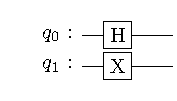
\includegraphics{images/4_Qiskit/example_circuit_1.pdf}
    \caption{Building a simple Quantum circuit and its diagram compiled from its \LaTeX source code}
\end{listing}


Qiskit also provides us with functions that can visualize a circuit. Every QuantumCircuit object has a member function for
printing the circuit using many different output methods like: ASCII text (great if you are in a CLI enviroment), as a Matplotlib
plot if you are in an interactive Python enviroment or output the \LaTeX source code of the circuit diagram for the highest resolution.
\section{Measuruments in Qiskit}

Measuring the outcome of the qubits in a Quantum circuit is very important in Quantum Computing because it allows us to verify our
algorithm quantitativily. Qiskit allows us to measure in two ways: measure a qubit into a specific bit or measure every qubit at once
into a classical register.

If we want to measure each qubit or group of qubit into specific bits or classical registers we must ensure to instanciate the circuit
object with the appropriate amount of bits. This can be done by passing an integer as the second parameter on instanciation. Then
we can specify which qubit line we want to measure into which bit line by invoking the \verb|measure()| member method of the circuit
object.

\begin{figure}[ht]
    \centering
    \begin{minted}{python3}
        from qiskit import QuantumCircuit

        circuit = QuantumCircuit(2, 2) # 2 qubits + 2 bits
        
        circuit.h(0)
        circuit.x(1)

        circuit.measure(0, 0) # measure q_0 and store the outcome on c_0
        circuit.measure(1, 1) # measure q_1 and store the outcome on c_1

        print(circuit.draw("latex_source"))
    \end{minted}
    \centering
    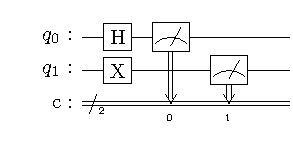
\includegraphics{images/4_Qiskit/example_meas_q2b_1.pdf}
    \caption{Measuring qubit states into the appropriate bits}
\end{figure}

Finally, if we want to measure all qubits at once we can invoke the \verb|measure_all()| member method of the circuit object.
Note that we do not need to specify how many bits the cirucit needs, Qiskit auto-calculates the appropriate amount and
supplies the circuit with a pre-allocated classical register named \verb|meas|.

\begin{figure}[ht]
    \begin{minted}{python3}
        from qiskit import QuantumCircuit
    
        circuit = QuantumCircuit(2, 2)
        
        circuit.h(0)
        circuit.x(1)
    
        circuit.measure_all() # measure everything in one batch
    
        print(circuit.draw("latex_source"))
    \end{minted}
    \centering
    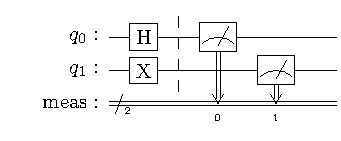
\includegraphics{images/4_Qiskit/example_meas_all_1.pdf}
    \caption{Measuring all the qubit outcomes of the circuit at once}
\end{figure}
\section{Custom Quantum Gates}

Qiskit let us create our own gates. This can be done by build the desired gate from the basis gate set supplied by the
Qiskit SDK and then invoke the \verb|to_gate()| member method of the circuit object. For example, we can create a new
gate $G$ from the circuit we created from the previous section. After we create the custom gate we can use the \verb|append|
member method to append it to our base circuit.

\begin{figure}[ht]
    \centering
    \begin{minted}{python3}
        from qiskit import QuantumCircuit
            
        example_circuit = QuantumCircuit(2, name="G")
            
        example_circuit.h(0)
        example_circuit.x(1)
            
        example_gate = example_circuit.to_gate()
            
        circuit = QuantumCircuit(2)
            
        circuit.append(example_gate, [0, 1])
        print(circuit.draw("latex_source"))
    \end{minted}
    \centering
    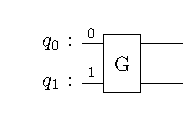
\includegraphics{images/4_Qiskit/example_custom_gate_1.pdf} 
    \caption{Creating a custom gate $G$ and appending it to another circuit}
\end{figure}
\section{Local Simulations, Transpilation and Sending a Job on a Real Quantum Computer}

After measuring the Quantum circuit we can use Qiskit to execute a Quantum circuit in two ways:

\begin{enumerate}
    \item execute it using a simulator on your local machine or
    \item send your circuit to be run as a \textit{job} on real Quantum hardware
\end{enumerate}

We are going to mention how to execute Quantum circuits using both ways.

IBM provides a high performance local simulator called \textit{Aer} (pronounced \textit{air}).
There are even two versions of the Aer simulator: a GPU-based simulator that can use a 
\textit{Graphics Processing Unit} to accelarate the simulation execution or a CPU-based
simulator. We are going to use the later and more specifically on a Intel i5 four core, eight thread
CPU. We did this as to prove that these kinds of circuits can run even on moderately modern hardware.


\subsection{The Aer Simulator}
For this example we will execute the simple Quantum circuit that we created on the previous sections.

Before importing anything we should install the \verb|Aer| simulation library. Again this is extremely
simple as we can use \verb|pip| to install those dependencies automatically. After the installation,
we can import the \verb|AerSimulator| class from the \verb|qiskit_aer| library we just installed and
instanciate it as an object named \verb|sim|.

We should note that to execute circuits with custom gate components we should \textit{transpile} the
circuit before executing it. Transpilation in Qiskit is the process of converting a Quantum circuit
using a simpler set of \textit{basis gates}. Transpilation is very important in Qiskit and it will 
come handy when we want to execute circuits on real Quantum computers. Transpilation is taken care
of by the \verb|transpile()| method from the \verb|qiskit| library. It takes two positional arguments:
the circuit(s) to be transpiled and the simulator that the circuit(s) will be transpiled for. Strictly
speaking this simple example circuit does not need any further simplification but for the purposes of
demonstrations we will transpile the circuit.

The final step is to invoke the \verb|run| member method of the instanciated simulator. We can also
invoke the \verb|result()| method right after the invokation of the \verb|run()| method to get back the
result counts of the execution.

\begin{listing}[ht]
    \centering
    \begin{minted}{python3}
        from qiskit_aer import AerSimulator
        from qiskit import transpile

        sim = AerSimulator()
        circuit = transpile(circuit, sim)
        result = sim.run(circuit).result()
    \end{minted}
    \caption{Executing the example Quantum circuit on a local CPU-based Aer simulator}
\end{listing}

The \textit{result counts} are the counts of the probabilities for each qubit in the Quantum circuit. The default
max count limit is 1024 and it can be changed accordingly. We will leave the default values.
To plot those result we will use the \verb|qiskit.visualization| library that comes with the base Qiskit installation.
The \verb|plot_histogram()| method plots the result as histogram where the x-axis is the output state of the Quantum
circuit and the y-axis is how many times this was the output. Note that to get the counts of the result invoke the 
\verb|get_counts()| method.

\begin{listing}[ht]
    \centering
    \begin{minted}{python3}
        from qiskit.visualization import plot_histogram
        plot_histogram(result.get_counts())
    \end{minted}
    \centering
    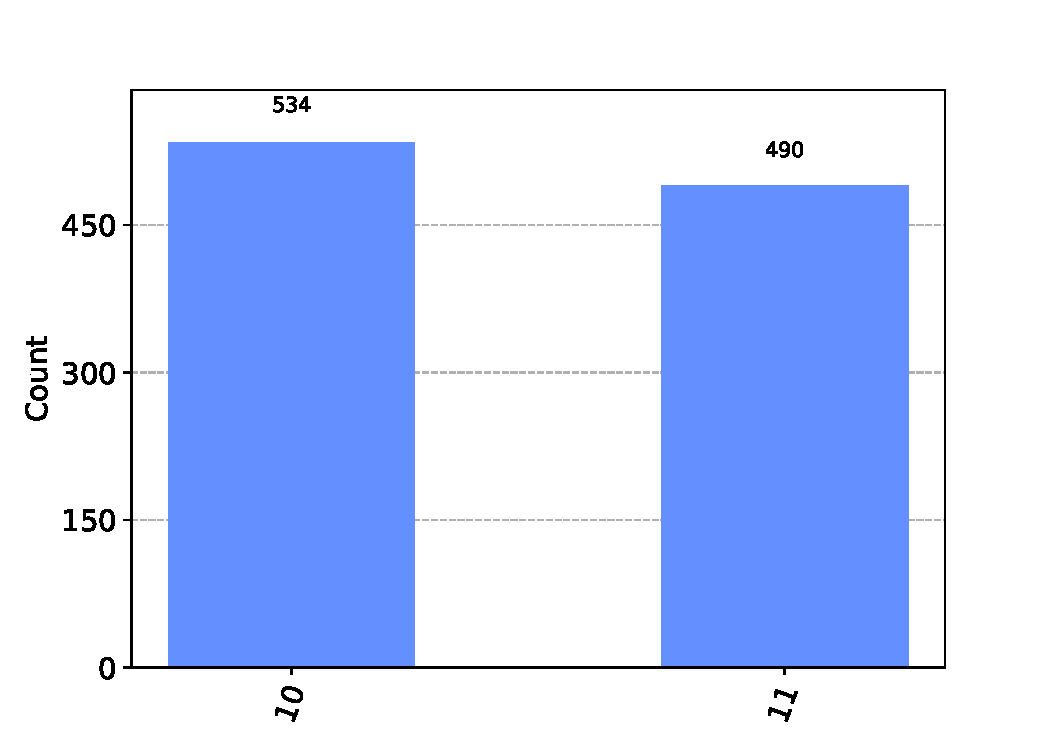
\includegraphics[scale=0.8]{images/4_Qiskit/example_circuit_counts_plot.pdf}
    \caption{The plotted result of the simualtion for the example circuit}
\end{listing}

We can see that on the x-axis we have two outputs: \verb|10| with a count of 534 and \verb|11| with a count
of 490 which count up to 1024. This means that qubit $q_0$ is $50\%$ of the time in the $\ket{0}$ state and
the other $~50\%$ of the time in the $\ket{1}$ state. This makes sense because we applied earlier a Hadamard
gate on the qubit putting it on superposition of those two basis states. As for $q_1$, for every qubit is initialized
to the $\ket{0}$ state, and by applying the $X$ gate we invert it from $\ket{0}$ to $\ket{1}$.

We would like to note that the bitstring label for each output in the histogram is represented in little-endian,
meaning that the first measurement of a qubit is going to be displayed as the least-significant bit of that label.

\subsection{Executing on a Real Quantum Computer}

In general, executing a Quantum circuit on a real Quantum computer is not much different than executing on a local
simulator, although, some additional steps are needed.

First of all, the IBM Quantum Platform provides users with nine different \textit{compute resources}, essential
Quantum computers that are avalaible for upto 10 minutes of compute time per month for each user. Each of these
Quantum computers are based on a different set of basis gates. For example, the \verb|ibm_osaka| computer
is based on IBM's Eagle r3 Quantum Processor, scoring 127 qubits in total and with basis gates: ECR, ID, RZ, SX
and X gates.

This means that for each Quantum computer, our circuit needs to be transpiled specificly in mind of the basis gates
of the \textit{target compute resource}.

On that note, an extra library must be installed on our system to configure the circuit to
be sent over the Internet to IBM's Quantum Platform, the \verb|QiskitRuntimeService|. This
is a trivial task, as it can be installed by \verb|pip|. After the installation, we can
instanciate a \verb|QiskitRuntimeService| object named \verb|service|. IBM recommends to
configure the service by saving your credentials (API Token) locally. This can be done by
invoking the \verb|save_account()| member method of the \verb|service| object. We can then
specify which \textit{channel}, or service, and \textit{token} (your acount's API token).
It is additionaly recommented to set the positional argument \verb|set_as_default| to
\mintinline{python3}|True|. We should note that this is an extremely unsafe operational
because anyone with access to our operating system user account has direct access to our
IBM Quantum Platform account.

After that everytime we instanciate a \verb|QuantumRuntimeService| object the configuration
is automatically set to use our credentials.

The next step is to find a Quantum computer to execute our circuit. Qiskit provides the very
handy \\\verb|least_busy()| member method, that finds the least busy backend (Quantum computer)
at that specific time. This method also can specify what kind of backend we may request, because
IBM provides also simulator in addition to real Quantum computers, with setting the positional
argument \verb|simulator| to \mintinline{python3}|False|.

The next step is the transpilation. IBM recommends to build a target-specific transpiler which
using the \verb|generate_preset_passmanager()| method from the \verb|qiskit.transpile| library.

This method can also be configured to optimize the circuit at a specific level by the
positional argument \\\verb|optimization_level| and set a target backend which will be used
to transpile the circuit to use the set of basis gates of that target.

After all the initializations and configurations we can run the transpiler with our circuit
by invoking the \verb|run| member method from the generated transpiler.

Finally, we have to instanciate a \textit{Qiskit primitive}. A Qiskit primitive is an abstraction
layer that lets users specify on a high-level settings to be passed onto the runtime without
implementing it by hand. We will use a pre-configured Qiskit primitive, the \textit{SampleV2}.
This primitive will configure the runtime to return the probabilities of the output qubits
of our circuit, something like the counts results we got from the previous subsection.

\begin{listing}[ht]
    \centering
    \begin{minted}{python3}
        from qiskit_ibm_runtime import QiskitRuntimeService
        from qiskit.transpiler.preset_passmanagers import
            generate_preset_pass_manager
        from qiskit_ibm_runtime import SamplerV2 as Sampler

        service = QiskitRuntimeService()
        backend = service.least_busy(operational=True, simulator=False)
        pm = generate_preset_pass_manager(optimization_level=1, backend=backend)
        circuit = pm.run([circuit])
        job = Sampler(backend).run([circuit])
        result = job.result()

        plot_histogram(result[0].data.meas.get_counts())
    \end{minted}
    \centering
    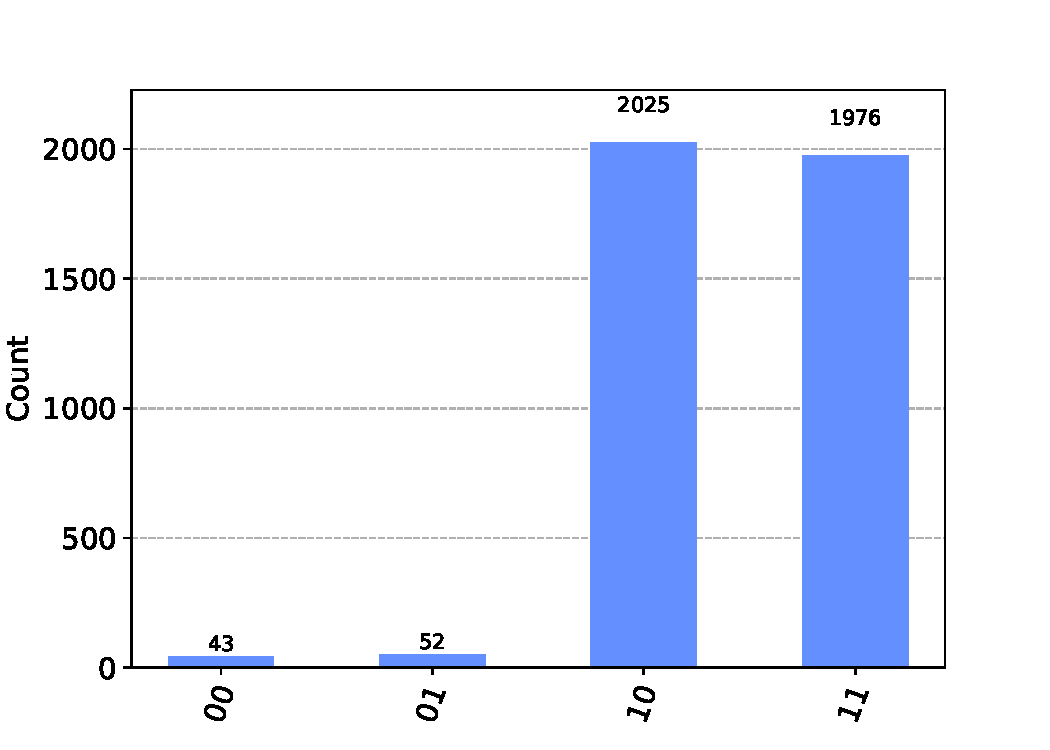
\includegraphics[scale=0.45]{images/4_Qiskit/example_circuit_counts_ibm_osaka.pdf}
    \caption{Executing the example circuit on the IBM Osaka Quantum Computer}
\end{listing}

As we can see two new bars appear seemingly out of nowhere. We can see that
$~0.01\%$ of the time the output is in the $\ket{00}$ state and $0.012\%$
of the time in the $\ket{01}$ state. This is expectable because modern state-of-the-art
Quantum computers are very susceptible to noise. This is a very good example of
this phenomenon, where noise introduces unexpected and unwanted behavior to our
system, where previously, when executed on a simulator, there was none of this
ouput. This is a very serious problem for scientists and engineers that
construct Quantum computers. Unfortunately, we are not going to cover noise
mitigitation strategies but this work could definitely benefit
from these kinds of strategies because as you introduce more qubits and more
gates onto your circuit design noise will affect the behavior of your system
over-all.